\documentclass[11pt,a4paper]{article}

\usepackage[T1]{fontenc}
\usepackage[utf8]{inputenc}
\usepackage{lmodern}
\usepackage{microtype}
\usepackage[margin=1in]{geometry}
\usepackage{amsmath,amssymb}
\usepackage{booktabs}
\usepackage{array}
\usepackage{multirow}
\usepackage{tocloft}
\setlength{\cftbeforesecskip}{0.3em}
\newcolumntype{L}[1]{>{\raggedright\arraybackslash}p{#1}}
\usepackage{siunitx}
\sisetup{group-separator={,}, group-minimum-digits=4}
\usepackage{threeparttable}
\usepackage{graphicx}
\usepackage{xcolor}
\usepackage[english]{babel}
\usepackage{csquotes}
\usepackage[style=apa,backend=biber,uniquename=init,maxcitenames=2]{biblatex}
\addbibresource{references.bib}
\usepackage[hidelinks]{hyperref}
\hypersetup{pdftitle={Detection Under an Alert Budget: A Leak-Free Case Study of Authentication Anomaly Detectors on the LANL Data, with a Reproduction of Euler},
  pdfauthor={Mahamane Sani Adamou Mahamane}, pdfsubject={AuthBench report, version 2},
  pdfkeywords={anomaly detection, authentication logs, alert budget, LANL, evaluation, reproducibility}}
\usepackage[capitalise,noabbrev]{cleveref}

% Generated by scripts/paper_assets.py from committed run outputs. Do not edit.
\newcommand{\WideTrainEvents}{133{,}093{,}586}
\newcommand{\WideTrainPositives}{50}
\newcommand{\WideTrainCampaigns}{11}
\newcommand{\WideTrainRate}{3.76 \times 10^{-7}}
\newcommand{\WideTrainTopHostPositives}{42}
\newcommand{\WideTrainTopHostCampaigns}{9}
\newcommand{\WideTrainTopHostShare}{84.0\%}
\newcommand{\WideTrainSourceHosts}{3}
\newcommand{\WideValEvents}{51{,}687{,}105}
\newcommand{\WideValPositives}{266}
\newcommand{\WideValCampaigns}{45}
\newcommand{\WideValRate}{5.15 \times 10^{-6}}
\newcommand{\WideValTopHostPositives}{261}
\newcommand{\WideValTopHostCampaigns}{45}
\newcommand{\WideValTopHostShare}{98.1\%}
\newcommand{\WideValSourceHosts}{2}
\newcommand{\WideTestEvents}{54{,}690{,}768}
\newcommand{\WideTestPositives}{282}
\newcommand{\WideTestCampaigns}{52}
\newcommand{\WideTestRate}{5.16 \times 10^{-6}}
\newcommand{\WideTestTopHostPositives}{275}
\newcommand{\WideTestTopHostCampaigns}{50}
\newcommand{\WideTestTopHostShare}{97.5\%}
\newcommand{\WideTestSourceHosts}{3}
\newcommand{\TopHost}{C17693}
\newcommand{\WideRandomRocAuc}{0.488}
\newcommand{\WideRandomAucPr}{5.05 \times 10^{-6}}
\newcommand{\WideRandomRecallAtFiveHundred}{0.0\%}
\newcommand{\WideRandomFirstDetection}{85{,}070}
\newcommand{\WideAlwaysFailRocAuc}{0.496}
\newcommand{\WideAlwaysFailAucPr}{5.16 \times 10^{-6}}
\newcommand{\WideAlwaysFailRecallAtFiveHundred}{0.0\%}
\newcommand{\WideAlwaysFailFirstDetection}{5{,}505{,}419}
\newcommand{\WidePairRarityRocAuc}{0.941}
\newcommand{\WidePairRarityAucPr}{7.75 \times 10^{-4}}
\newcommand{\WidePairRarityRecallAtFiveHundred}{0.0\%}
\newcommand{\WidePairRarityFirstDetection}{2{,}852}
\newcommand{\WidePcaRocAuc}{0.930}
\newcommand{\WidePcaAucPr}{3.50 \times 10^{-5}}
\newcommand{\WidePcaRecallAtFiveHundred}{0.0\%}
\newcommand{\WidePcaFirstDetection}{1{,}569}
\newcommand{\WideIForestRocAuc}{0.876}
\newcommand{\WideIForestAucPr}{1.92 \times 10^{-5}}
\newcommand{\WideIForestRecallAtFiveHundred}{0.0\%}
\newcommand{\WideIForestFirstDetection}{141{,}522}
\newcommand{\WideHbosRocAuc}{0.884}
\newcommand{\WideHbosAucPr}{3.32 \times 10^{-5}}
\newcommand{\WideHbosRecallAtFiveHundred}{0.0\%}
\newcommand{\WideHbosFirstDetection}{104{,}963}
\newcommand{\WideRulesRocAuc}{0.563}
\newcommand{\WideRulesAucPr}{4.69 \times 10^{-4}}
\newcommand{\WideRulesRecallAtFiveHundred}{0.0\%}
\newcommand{\WideRulesFirstDetection}{999}
\newcommand{\OnedayRandomRocAuc}{0.500}
\newcommand{\OnedayRandomAucPr}{1.12 \times 10^{-5}}
\newcommand{\OnedayRandomRecallAtFiveHundred}{0.0\%}
\newcommand{\OnedayAlwaysFailRocAuc}{0.496}
\newcommand{\OnedayAlwaysFailAucPr}{1.04 \times 10^{-5}}
\newcommand{\OnedayAlwaysFailRecallAtFiveHundred}{0.0\%}
\newcommand{\OnedayPairRarityRocAuc}{0.942}
\newcommand{\OnedayPairRarityAucPr}{6.55 \times 10^{-4}}
\newcommand{\OnedayPairRarityRecallAtFiveHundred}{0.0\%}
\newcommand{\OnedayPcaRocAuc}{0.892}
\newcommand{\OnedayPcaAucPr}{4.62 \times 10^{-5}}
\newcommand{\OnedayPcaRecallAtFiveHundred}{0.0\%}
\newcommand{\OnedayIForestRocAuc}{0.872}
\newcommand{\OnedayIForestAucPr}{4.02 \times 10^{-5}}
\newcommand{\OnedayIForestRecallAtFiveHundred}{0.0\%}
\newcommand{\OnedayHbosRocAuc}{0.875}
\newcommand{\OnedayHbosAucPr}{5.41 \times 10^{-5}}
\newcommand{\OnedayHbosRecallAtFiveHundred}{0.0\%}
\newcommand{\OnedayRulesRocAuc}{0.547}
\newcommand{\OnedayRulesAucPr}{9.85 \times 10^{-5}}
\newcommand{\OnedayRulesRecallAtFiveHundred}{5.1\%}
\newcommand{\DemoRandomRocAuc}{0.497}
\newcommand{\DemoRandomAucPr}{1.56 \times 10^{-3}}
\newcommand{\DemoRandomRecallAtFiveHundred}{50.0\%}
\newcommand{\DemoRandomFirstDetection}{162}
\newcommand{\DemoAlwaysFailRocAuc}{0.491}
\newcommand{\DemoAlwaysFailAucPr}{1.37 \times 10^{-3}}
\newcommand{\DemoAlwaysFailRecallAtFiveHundred}{75.0\%}
\newcommand{\DemoAlwaysFailFirstDetection}{165}
\newcommand{\DemoPairRarityRocAuc}{0.477}
\newcommand{\DemoPairRarityAucPr}{2.46 \times 10^{-3}}
\newcommand{\DemoPairRarityRecallAtFiveHundred}{25.0\%}
\newcommand{\DemoPairRarityFirstDetection}{294}
\newcommand{\DemoPcaRocAuc}{0.783}
\newcommand{\DemoPcaAucPr}{4.05 \times 10^{-3}}
\newcommand{\DemoPcaRecallAtFiveHundred}{75.0\%}
\newcommand{\DemoPcaFirstDetection}{114}
\newcommand{\DemoIForestRocAuc}{0.798}
\newcommand{\DemoIForestAucPr}{4.20 \times 10^{-3}}
\newcommand{\DemoIForestRecallAtFiveHundred}{75.0\%}
\newcommand{\DemoIForestFirstDetection}{282}
\newcommand{\DemoEcodRocAuc}{0.690}
\newcommand{\DemoEcodAucPr}{4.57 \times 10^{-3}}
\newcommand{\DemoEcodRecallAtFiveHundred}{50.0\%}
\newcommand{\DemoEcodFirstDetection}{83}
\newcommand{\DemoRulesRocAuc}{0.911}
\newcommand{\DemoRulesAucPr}{3.31 \times 10^{-1}}
\newcommand{\DemoRulesRecallAtFiveHundred}{100.0\%}
\newcommand{\DemoRulesFirstDetection}{1}
\newcommand{\WideSpearmanRocAuc}{-0.10}
\newcommand{\WideKendallRocAuc}{0.00}
\newcommand{\WideSpearmanAucPr}{0.70}
\newcommand{\WideKendallAucPr}{0.60}
\newcommand{\DemoSpearmanRocAuc}{0.60}
\newcommand{\DemoKendallRocAuc}{0.40}
\newcommand{\DemoSpearmanAucPr}{0.90}
\newcommand{\DemoKendallAucPr}{0.80}
\newcommand{\WideNonTrivialModels}{5}
\newcommand{\WidePairsTotal}{21}
\newcommand{\WidePairsSignificant}{18}
\newcommand{\WidePairsAtFloor}{18}
\newcommand{\WideHolmFloor}{0.0210}
\newcommand{\OnedayPairsTotal}{21}
\newcommand{\OnedayPairsSignificant}{13}
\newcommand{\OnedayPairsAtFloor}{12}
\newcommand{\OnedayHolmFloor}{0.0210}
\newcommand{\DemoRSevenRatio}{114}
\newcommand{\DemoRSevenWeight}{0.521}
\newcommand{\WideFloorTieContenders}{413{,}567}

\makeatletter
\newcommand{\tablerows}[1]{\@@input #1 }
\makeatother

\newcommand{\AuthBench}{\textsc{AuthBench}}
\newcommand{\Rcamp}{R_{\mathrm{camp}}}
\newcommand{\Rev}{R_{\mathrm{ev}}}

\title{Detection Under an Alert Budget:\\
A Leak-Free Case Study of Authentication Anomaly Detectors\\
on the LANL Data, with a Reproduction of Euler}

\author{Mahamane Sani Adamou Mahamane\\[2pt]
\small University of the People\\
\small \href{mailto:saniadamou778@gmail.com}{\texttt{saniadamou778@gmail.com}}\\
\small ORCID \href{https://orcid.org/0009-0001-5561-753X}{0009-0001-5561-753X}}

\date{October 2026}

\begin{document}
\maketitle

\begin{abstract}
\noindent Security operations centres investigate a bounded number of alerts per day, yet anomaly detectors for authentication logs are mostly compared by threshold-free metrics. We present \AuthBench{}, an open evaluation harness that enforces its temporal split in code, scores every event independently of the others, ranks events within each day, and reports for each red-team campaign the daily budget at which it is first detected, with the exact distribution of that budget under a random ranking. We evaluate rules, rarity scores, outlier detectors, two autoencoders and a reimplementation of the temporal graph detector Euler on the authentication log of the Los Alamos National Laboratory (LANL) data, under the harmonised protocol of Larroche (training on the first 41 hours, testing on the next 57 days, no labels; \HarmTestPositives{} red-team events in \HarmTestCampaigns{} campaigns) and under a day-based split. Ranked as individual events, no detector detects a campaign at 10 alerts per day, and none exceeds \TempPcaRecallFiveHundred{} of the campaigns at 500. In the harmonised protocol, the detectors whose first detection a random ranking rarely matches (PCA, the VAE and the autoencoder, at \HarmPcaFirstDetection{}, \HarmVaeFirstDetection{} and \HarmAutoencoderFirstDetection{} alerts per day) are not those with the highest ROC-AUC: over the non-trivial detectors, ROC-AUC and the first-detection budget are unrelated (Spearman $\rho = \HarmSpearmanRocAuc$ and $\TempSpearmanRocAuc$ in the two protocols). Ranked as user-days instead of events, Euler and a source-novelty score reach about half of the campaigns at 500 per day, against \HarmRandomUserDayFiveHundred{} for a random ranking: the alert unit matters as much as the detector. PCA's first detection ranges from \HarmPcaFitFirstMin{} to \HarmPcaFitFirstMax{} alerts per day over five fitting seeds. Rerun on the same machine, the authors' Euler code reproduces its published AUC (\EulerAuthorsAuc{} against \EulerPublishedAuc{}) but not its average precision (\EulerAuthorsAp{} against \EulerPublishedAp{}); our reimplementation reaches \EulerFidNtlmAuc{} and \EulerFidNtlmAp{} on an identical test set. The labelled activity is one intrusion, \RedTeamTopHostShare{} of it from one host, so these results are a case study of one operation, not an estimate for detectors in general.
\end{abstract}

% Table of contents on a page of its own, for the preprint; a venue's template replaces it.
\clearpage
\tableofcontents
\clearpage

\section{Introduction}
\label{sec:introduction}

An anomaly detector deployed in an enterprise network is consumed through an alert queue. Each day, analysts investigate the highest-ranked alerts until their capacity is exhausted, and the detector is useful only if an attack appears within that capacity. Interviews with SOC practitioners describe alert streams dominated by false positives \parencite{alahmadi2022}; automated triage has been proposed to combat the resulting alert fatigue \parencite{hassan2019nodoze}, and a lateral-movement detector deployed in a real enterprise has been reported at fewer than nine alerts per day \parencite{ho2021hopper}. The base-rate argument of \textcite{axelsson2000} explains the constraint: when attacks are rare, even a small false-positive rate produces an alert stream dominated by false alarms.

Authentication logs are an extreme instance of this regime: in the harmonised test partition used here, the positive rate is $\HarmTestRate$. Detectors for such data are nevertheless often summarised by the area under the ROC curve (ROC-AUC), which averages the ranking over every operating point, including those no SOC could staff. That ROC-AUC is uninformative about the extreme left of the curve is the classical motivation for partial ROC areas \parencite{mcclish1989} and precision-recall analysis \parencite{davis2006,saito2015}, and it has been stated for the LANL data in particular \parencite{king2022euler}. Budget-based metrics have also been reported on LANL \parencite{larroche2021decades,garchery2020adsage,larroche2025ultralmd}. This paper does not claim the observation; it contributes a harness that makes the measurement reproducible and leak-free, and a case study whose limits are measured rather than assumed.

Our contributions are:
\begin{enumerate}
\item \textbf{An open evaluation harness} (\cref{sec:protocol,sec:evaluation}). It enforces the temporal split by code and tests that every detector scores an event identically alone or among others; ranks events, edge-hours and user-days within each day with a stated, label-free tie order and tie brackets; gives every campaign its detection budget, hence the whole campaign-recall curve, and the exact distribution of the first-detection budget under a random ranking; and reports a paired account-level bootstrap with BCa intervals and Monte Carlo errors, a bootstrap over source users, the variance of refitting with other seeds, a fixed-threshold deployment, and a staffing model for the budgets.
\item \textbf{A case study on LANL} (\cref{sec:results}) of thirteen detectors, from floors and rules to autoencoders and a temporal graph detector, under the protocol recommended by \textcite{larroche2026fair} and under a day-based split with and without red-team events in training.
\item \textbf{A reproduction of Euler} (\cref{sec:euler}) with the authors' own code run beside our reimplementation, and an edge-by-edge reconciliation of the two test sets with the published counts.
\item \textbf{Diagnostics that bound the case study} (\cref{sec:diagnostics,sec:circularity}): the concentration of the red-team events on one host, a rule-by-rule decomposition of the rule engine on LANL, and a control for circularity between a data generator and a rule.
\end{enumerate}

\section{Related work}
\label{sec:related}

\paragraph{Evaluation pitfalls in security machine learning.}
\textcite{axelsson2000} established the base-rate fallacy for intrusion detection, and \textcite{sommer2010} argued that anomaly detection differs from the closed-world settings in which machine learning usually succeeds. \textcite{pendlebury2019} showed that spatial and temporal experimental bias inflates malware classification results. \textcite{arp2022} identified ten recurring pitfalls, among them data snooping, inappropriate performance measures and the base-rate fallacy, and \textcite{apruzzese2023sok} assessed the practical value of machine learning for network intrusion detection. Leakage in data mining is formalised by \textcite{kaufman2012leakage}.

\paragraph{Metrics under class imbalance.}
ROC-AUC is invariant to the class ratio, whereas precision is not; \textcite{davis2006} related the two curves, and \textcite{saito2015} showed empirically that the precision-recall plot is the more informative one on imbalanced data. Partial ROC areas restrict the analysis to low false-positive rates \parencite{mcclish1989}. None of these encodes a capacity per unit of time, which is what an alert budget imposes.

\paragraph{Detection on the LANL data.}
The LANL comprehensive cyber-security events data \parencite{kent2015dataset,kent2016chapter} pairs 58 days of enterprise authentication events with labelled red-team activity; its authentication graph is characterised by \textcite{kent2015authgraphs}. \textcite{turcotte2016} model users relative to peer groups by Poisson factorisation. \textcite{tuor2018} apply recurrent language models to log lines; their operational metric is the average percentile of malicious events in a daily ranking, not average precision, and \textcite{brown2018} add attention mechanisms to that family. \textcite{bowman2020} learn node embeddings on the authentication graph, training on 40 days without reported malicious activity and testing on the 18 days with it, a split that is not chronological. \textcite{king2022euler} cast lateral-movement detection as temporal link prediction (Euler), train on the snapshots that precede the first anomalous edge, and note that ROC-AUC is not a good indicator of model quality on data as imbalanced as LANL. \textcite{xu2024argus} (Argus), \textcite{paudel2022pikachu} (Pikachu), \textcite{amin2019cadence} (CADENCE) and \textcite{gokstorp2024} (transformer sequence models) propose further detectors. Outside LANL, \textcite{siadati2017} detect structurally anomalous logins in an enterprise network.

\paragraph{Budgeted evaluation and recent re-evaluations.}
Daily-budget recall was used by \textcite{tuor2017} on insider-threat data and adopted by \textcite{garchery2020adsage}, who report cumulative recall over budgets of investigated user-days on LANL (training on days 1--8, testing on days 9--13) and find that a rule flagging previously unseen source computers performs on par with their graph-based detector. \textcite{larroche2021decades} keep remote LogOn events whose destination is a user account, train on 8 days and evaluate on the next 5, and report the detection rate for a fixed daily budget of investigated events (DR-1K, 1{,}000 events per day, of 0.081 for their detector) alongside a truncated ROC area. \textcite{larroche2025ultralmd} reports ROC-AUC, average precision and the recall obtained when the top $B$ edges of each hourly window are investigated; in his comparison, higher ROC-AUC does not imply higher budgeted recall. Two 2026 studies re-evaluate published detectors under harmonised conditions. \textcite{larroche2026fair} harmonises the preprocessing and labelling of LANL and OpTC and shows that published average precision values do not survive (for Argus on LANL, 32.27 as originally reported against $0.09 \pm 0.04$ re-evaluated, both in percent in his Table~5); he notes that the labelled LANL authentications belong to a single intrusion, mostly from one source host, recommends training on the first 41 hours and testing on the remainder with all remote LogOn events, and concludes that the dataset should be used only for unsupervised methods. \textcite{zhao2026gids} decompose graph-based intrusion detectors into interchangeable stages and find that an encoder-free control ranks first by average precision on two of four datasets.

\paragraph{Positioning.}
\AuthBench{} scores individual authentication events, ranks them within each day in three alert units, and counts detections per red-team campaign; it compares rules, statistical scores, outlier detectors, autoencoders and a temporal graph detector under one leak-free protocol, and places each first-detection budget against its distribution under a random ranking. Its event universe and units overlap with, but do not equal, those of the works above (\cref{sec:comparison}).

\section{Data, labels and campaigns}
\label{sec:data}

\subsection{Source}
We use the authentication log of the LANL comprehensive cyber-security events data \parencite{kent2015dataset}: 1{,}051{,}430{,}459 events over 58 days from one enterprise Windows Active Directory environment, with one-second timestamps from an arbitrary epoch. The official server refused connections when this run was prepared, so the files were taken from a public mirror; their compressed bytes differ from the official digests, and their content was verified instead: the row count is the published one, and three days have the row counts and order-independent content hashes of a conversion of the official files. Missing authentication and logon types are encoded as indicators. Failed authentications appear only for users who succeed at least once, so no conclusion is drawn about attacks on non-existent accounts.

\subsection{Labels and campaigns}
The red-team file contains 749 lines, of which 34 are exact duplicates, leaving \RedTeamRows{} distinct red-team events. Authentication events are labelled malicious by an exact join on the four red-team fields: time, user (with domain), source computer and destination computer; \RedTeamUnmatched{} red-team events have no authentication event at the same second between the same computers and cannot be labelled by any pipeline (\cref{sec:euler}). Red-team activity spans days 1 to 29. We group red-team events into campaigns per user: consecutive events of the same user belong to one campaign when they are at most $g = 24$ hours apart, and campaigns are cut at partition boundaries.

\subsection{Concentration of the red-team activity}
\label{sec:concentration}
Of the \RedTeamRows{} distinct red-team events, \RedTeamTopHostEvents{} (\RedTeamTopHostShare{}) start from one source computer, \TopHost{}, and only \RedTeamSourceComputers{} source computers appear at all; in the day-based test partition the share is \TempTestTopHostShare{} of the positives and \TempTestTopHostCampaigns{} of the \TempTestCampaigns{} campaigns. This agrees with the observation of \textcite{larroche2026fair} that the labelled LANL authentications belong to a single simulated intrusion. Our campaigns are therefore accounts and phases of one operation, not independent attacks, and the effective number of independent intrusions in this evaluation is one.

\section{Protocol}
\label{sec:protocol}

\subsection{Two protocols}
\label{sec:split}
\Cref{tab:split} gives both protocols. The \emph{harmonised} protocol follows \textcite{larroche2026fair}: training on hours 0 to 41, which end before the first red-team event (hour 41.9), and testing on every later hour of the data, with every event compared with all earlier events from day 0 and the universe restricted to remote LogOn events (source and destination computers differ). It has no validation partition, so no detector is tuned and no label is read anywhere. The \emph{temporal} protocol trains on days 0--7, validates on days 8--10 and tests on days 11--13, keeps every authentication event, and lets each partition read the two preceding days as warm-up; it is the configuration of the previous version of this report, rerun with the current code. Its partitions are those of that run, which the event counts confirm (\cref{app:earlier}). Day 11 holds no red-team event, so its test positives fall on days 12 (\TempTestDayTwelvePositives{}) and 13 (\TempTestDayThirteenPositives{}).

\begin{table}[t]
\centering
\small
\begin{threeparttable}
\caption{The two protocols. Positives are labelled red-team authentication events.}
\label{tab:split}
\begin{tabular}{llllrrr}
\toprule
Protocol & Partition & Period & Events & Positives & Campaigns & Positive rate \\
\midrule
\tablerows{generated/table_split.tex}
\bottomrule
\end{tabular}
\end{threeparttable}
\end{table}

\paragraph{Training regimes.} With training data that contain red-team events (temporal training holds \TempTrainPositives{}), a detector can be fitted with them, the situation of a defender who does not know the network is compromised (R1, reported), or without them (R2). Features are computed with the red-team events in both regimes, because the history an event is compared against cannot be cleaned by a defender who has not found the attack. In the harmonised protocol the two regimes coincide.

\subsection{Leakage control and row-locality}
\label{sec:leakage}
A guard raises an error unless the last training timestamp precedes the first validation timestamp and the last validation timestamp precedes the first test timestamp. A static architecture test fails if any module under \texttt{models/} or \texttt{features/} imports the only function that loads the test partition. Windowed features use causal primitives over $[t-w, t)$, and every quantity fitted for features or detectors (category frequencies, rule normalisations, empirical distributions, thresholds) is fitted on training data, or on validation for tuning.

The test partition is scored one day at a time, so each detector must give an event the same score alone, in any chunk and in the whole partition. A unit test asserts this to the last bit for every detector, and every scored day re-checks it on the positives: a tolerance would hide a one-ULP difference that moves an event across a tie. Matrix products whose summation order follows the batch shape are evaluated row by row for that reason. One element remains retrospective within a day: the daily top-$k$ is computed from all the events of the day. \Cref{sec:fixed} replaces it by a threshold fixed in advance.

\subsection{Features}
\label{sec:features}
Detectors that consume a feature vector receive 25 columns from four families (\cref{app:features}): event-level indicators and training-fitted category frequencies (F1); per-user event counts and failure ratios over the preceding hour and day (F2); novelty and rarity of three relations, (user, destination), (user, source) and (source, destination) (F3); and the time of day with the deviation of an event from its user's running circular mean (F4). Rarity is $-\log\bigl((k+1)/(n+1)\bigr)$ with $k$ the earlier occurrences of the relation and $n$ counted on days before the event's day, so equally novel events of one day tie instead of being ordered by their time. Features are computed one day at a time with the state carried from day to day, and equal those computed over the whole window to the last bit.

\section{Detectors}
\label{sec:detectors}

\Cref{tab:detectors} summarises the catalogue. The vector-space detectors and the autoencoders are fitted on a seeded sample of at most \num{5000000} training events, Euler on every training edge; every test event is scored. In the temporal protocol, each detector with a hyperparameter to choose (M1's rule weights, PCA's retained variance, Isolation Forest's forest and sample sizes, HBOS's bins and tolerance) receives the same budget of 20 candidates, its default among them, and keeps the one with the highest validation AUC-PR; the autoencoders and Euler are not tuned. M1u reports the same rules with uniform weights and no label, which separates what the rules detect from what choosing their weights on labels adds.

\begin{table}[t]
\centering
\small
\begin{threeparttable}
\caption{The detector catalogue. Every detector scores an event independently of the other events scored (\cref{sec:leakage}).}
\label{tab:detectors}
\begin{tabular}{@{}lp{9.2cm}c@{}}
\toprule
Detector & Definition & Labels \\
\midrule
M0a random & Uniform score from a seeded hash of the event identifier (floor) & no \\
M0b always-fail & 1 for a failed authentication, 0 otherwise (floor) & no \\
M1 rules & Eight rules (\cref{app:rules}), each mapped through an empirical CDF fitted on the last training day, combined by a weighted sum; weights tuned on validation AUC-PR (temporal) & validation \\
M1u rules, uniform & The same rules with uniform weights & no \\
M2a pair rarity & Rarity of the (user, destination) pair & no \\
M2c source rarity & Rarity of the (user, source) pair, the \enquote{known source pc} signal of \textcite{garchery2020adsage} & no \\
M2b PCA & Mean squared reconstruction error of standardised features under PCA \parencite{lakhina2004} & no \\
M3a Isolation Forest & \parencite{liu2008iforest} & no \\
M3b HBOS & Histogram-based outlier score \parencite{goldstein2012hbos} & no \\
M3c ECOD & Empirical-CDF outlier score \parencite{li2022ecod}, distributions fitted on training data & no \\
M4a autoencoder & Dense autoencoder (64, 16, 64), mean squared reconstruction error & no \\
M4b VAE & Variational autoencoder \parencite{kingma2014vae} (64, 16, latent 8), negative ELBO at the posterior mean & no \\
M5c Euler & Reimplementation of \textcite{king2022euler}: GCN \parencite{kipf2017gcn} and GRU over 30-minute snapshots of the computer graph, edge scored from the previous snapshot's embeddings (\cref{sec:euler}) & no \\
\bottomrule
\end{tabular}
\begin{tablenotes}\footnotesize
\item M3a, M3b and M3c use the implementations of PyOD \parencite{zhao2019pyod}, M3c refitted so that its scores do not depend on the scored matrix. In the code and the run outputs, M3b is \texttt{M3b\_hbos} and M3c is \texttt{M3b\_ecod}. The autoencoders train for at most 30 epochs with early stopping on a 10\% holdout.
\end{tablenotes}
\end{threeparttable}
\end{table}

Euler sees every edge of the timeline before scoring the next snapshot, as a deployed Euler would: it is trained on the training rows, run once along the whole timeline, and scores an event by the negated log-odds of its edge under the previous snapshot's embeddings. Choices the paper does not fix are ours and are stated in the code: dropout 0.1, learning rate 0.01 from its grid, at most 100 epochs with patience 10, back-propagation truncated to one day, and one shared node for computers unseen in training.

\section{Evaluation}
\label{sec:evaluation}

\subsection{Budgeted metrics}
Let $E_d$ be the events of test day $d$, $P$ the red-team events and $\mathcal{C}$ the campaigns, each a set $P_c \subseteq P$. A detector assigns a score $s(e)$ to every event. Within each day, events are ordered by decreasing score, ties being ordered by arrival (time, then event identifier), an order that is total and independent of labels. Let $r(e)$ be the rank of $e$ in its day. The alert set at daily budget $k$ is $A(k) = \{\, e : r(e) \le k \,\}$, and event and campaign recall are
\begin{equation}
\Rev(k) = \frac{|A(k) \cap P|}{|P|}, \qquad
\Rcamp(k) = \frac{|\{\, c \in \mathcal{C} : P_c \cap A(k) \neq \emptyset \,\}|}{|\mathcal{C}|}.
\end{equation}
With the detection budget of a campaign $b(c) = \min_{e \in P_c} r(e)$, a campaign is detected at budget $k$ exactly when $b(c) \le k$, so $\Rcamp$ is the empirical distribution function of $\{b(c)\}$ (\cref{fig:recall}). We report $k \in \{10, 50, 100, 500\}$ and the first-detection budget $b^{*} = \min_{c} b(c)$, the smallest daily budget at which a detector detects anything; it does not saturate at zero where recall at a fixed budget does.

\paragraph{Random-ranking null.} For a uniformly random ranking, the positives of day $d$ occupy a uniformly random subset of $p_d$ ranks among $N_d$, so
\begin{equation}
\Pr\bigl(b^{*} > x\bigr) = \prod_{d} \binom{N_d - x}{p_d} \Big/ \binom{N_d}{p_d}.
\end{equation}
Its median is \HarmNullFirstDetectionMedian{} alerts per day in the harmonised test and \TempNullFirstDetectionMedian{} in the temporal test, with central 95\% ranges [\HarmNullFirstDetectionLow{}, \HarmNullFirstDetectionHigh{}] and [\TempNullFirstDetectionLow{}, \TempNullFirstDetectionHigh{}]. We report, for each detector, the exact null probability $\Pr(b^{*}_{\mathrm{random}} \le b^{*})$ rather than comparing with the single realisation of the random floor M0a.

\paragraph{Ties.} For coarse scores, which events enter $A(k)$ can depend on the tie order rather than the detector. We report $\Rcamp(k)$ under the stated arrival order with a bracket: the least favourable order (benign first within each tied group) and an achievable favourable one, with the number of tied events competing for the last places.

\paragraph{Alert units.} Analysts rarely triage single events. Every run also ranks two coarser units per day: the \emph{edge-hour} (source computer, destination computer, hour) and the \emph{user-day} (source user). A unit takes the score of its highest event; equal units are ordered by their first event's time, then by key, which reads no label, and no tie bracket is computed for units. A campaign is detected at budget $k$ in a unit when one of its units ranks in the top $k$ of its day. Units are fewer than events (between \HarmUserDaysMin{} and \HarmUserDaysMax{} user-days per harmonised test day), so the same $k$ covers a larger share of each day.

\paragraph{What a budget costs.} With 2.7 hours of triage per analyst and day \parencite{vectra2023} and 10 to 20 minutes per alert \parencite{li2026sheragent}, 10 alerts per day take \StaffTenLow{} to \StaffTenHigh{} analysts, 100 take \StaffHundredLow{} to \StaffHundredHigh{}, and 500 take \StaffFiveHundredLow{} to \StaffFiveHundredHigh{}, about a third of the alerts a typical SOC handles in a day across all its tools. Both inputs are weak (a vendor-commissioned survey and a self-reported preprint), but they place 10 alerts per day at one analyst and 500 at a team, not at equally plausible operating points.

\subsection{Threshold-free and low-false-positive-rate metrics}
ROC-AUC averages the ranking over all operating points. The area under the precision-recall curve (AUC-PR), estimated by average precision over the test partition, weights each positive by the precision at its rank and is therefore dominated by the best-ranked positives. Recall at a false-positive rate of $10^{-4}$, computed over the whole test partition, concerns only the top of the ranking.

\subsection{Uncertainty}
\label{sec:uncertainty}
Events of a campaign are dependent, and two campaigns of one account are not independent either, so we resample blocks \parencite{efron1993,field2007}: compromised accounts, each with all its red-team events, and individual benign events, drawn with replacement and with every detector evaluated on the same resamples. Resamples without positives are discarded and redrawn. With $R = \num{10000}$ resamples, each detector's AUC-PR receives a BCa interval \parencite{efron1987} whose acceleration comes from the exact jackknife over every resampling unit, and each pairwise difference a percentile interval and the sign statistic
\begin{equation}
p = \min\!\left(1, \frac{2\,(t+1)}{R+1}\right), \qquad t = \min\bigl(\#\{\Delta^{*} \le 0\}, \#\{\Delta^{*} \ge 0\}\bigr),
\end{equation}
corrected over the 78 pairs by the procedure of \textcite{holm1979}; every interval endpoint and $p$-value carries its Monte Carlo error. The first-detection budget and the other campaign-budget summaries are resampled over accounts too; because $b^{*}$ is a minimum, a resample can lose its best campaign but never beat it, so the lower end of its percentile interval equals the point value and the interval is one-sided.

Two variances escape this bootstrap. The benign events of one user are correlated, so the analysis is repeated with source users as the resampling unit, every event of a user moving with it. And the fitted detectors are held fixed: M1, PCA, Isolation Forest, ECOD and HBOS are refitted with five seeds, their tuned configuration fixed, to measure what another fit would change. The autoencoders and Euler are fitted once.

\subsection{A fixed threshold}
\label{sec:fixed}
No SOC tool ranks a day after it ends. For each budget $k$, the threshold at which the calibration partition raised $k$ alerts per day on average is applied to the test partition, where the alert volume then varies from day to day. Calibration uses validation in the temporal protocol and training in the harmonised one; it reads volumes, never labels.

\section{Results}
\label{sec:results}

\Cref{tab:results-harmonised,tab:results-temporal} report the two protocols, \cref{fig:first-detection} places every first-detection budget against ROC-AUC, AUC-PR and the null, and \cref{fig:recall} gives the whole campaign-recall curves.

\begin{table}[t]
\centering
\footnotesize
\begin{threeparttable}
\caption{Harmonised protocol (\HarmTestDays{} test days, \HarmTestCampaigns{} campaigns over \HarmTestAccounts{} accounts). R@$10^{-4}$: recall at a false-positive rate of $10^{-4}$. @50, @500: campaign recall at 50 and 500 alerts per day. $b^{*}$: first-detection budget, in alerts per day. Null: probability that a random ranking does at least as well.}
\label{tab:results-harmonised}
\setlength{\tabcolsep}{2pt}
\begin{tabular}{@{}lllrrrrrr@{}}
\toprule
Detector & AUC-PR & 95\% BCa interval & ROC-AUC & R@$10^{-4}$ & @50 & @500 & $b^{*}$ & Null \\
\midrule
\tablerows{generated/table_results_harmonised.tex}
\bottomrule
\end{tabular}
\begin{tablenotes}\footnotesize
\item Campaign recall is 0 for every detector at 10 alerts per day. Without validation, M1 keeps uniform weights and equals M1u. M2a's recall depends on the tie order (\cref{sec:ties-results}); every other bracket has zero width except M0b's.
\end{tablenotes}
\end{threeparttable}
\end{table}

\begin{table}[t]
\centering
\footnotesize
\begin{threeparttable}
\caption{Temporal protocol, regime R1 (test days 11--13, \TempTestCampaigns{} campaigns over \TempTestAccounts{} accounts). Columns as in \cref{tab:results-harmonised}.}
\label{tab:results-temporal}
\setlength{\tabcolsep}{2pt}
\begin{tabular}{@{}lllrrrrrr@{}}
\toprule
Detector & AUC-PR & 95\% BCa interval & ROC-AUC & R@$10^{-4}$ & @50 & @500 & $b^{*}$ & Null \\
\midrule
\tablerows{generated/table_results_temporal.tex}
\bottomrule
\end{tabular}
\begin{tablenotes}\footnotesize
\item Campaign recall at 10 alerts per day is 0 for every detector. M1's weights are tuned on validation labels; M1u reads no label.
\end{tablenotes}
\end{threeparttable}
\end{table}

\begin{figure}[t]
\centering
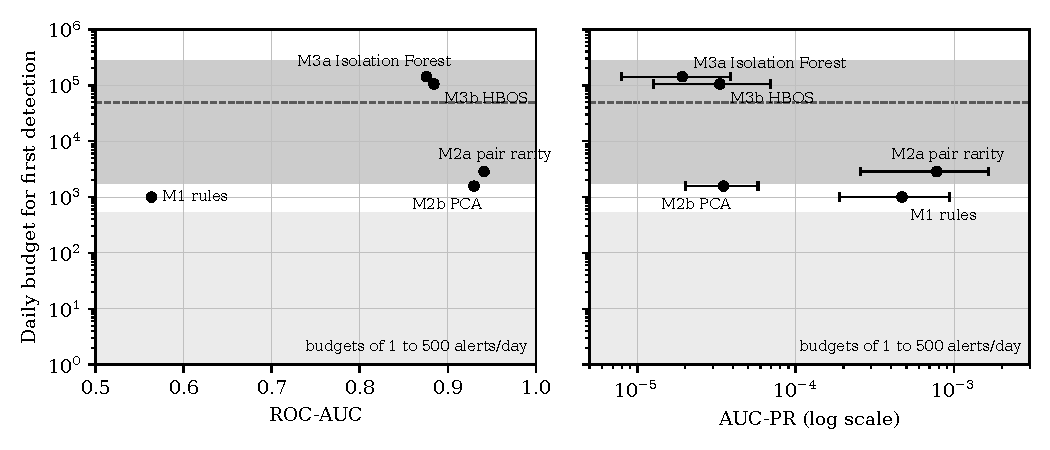
\includegraphics[width=\textwidth]{generated/figure_first_detection.pdf}
\caption{First-detection budget against ROC-AUC (left) and AUC-PR with its 95\% BCa interval (right), harmonised protocol (top) and temporal protocol (bottom), for the non-floor detectors. Dark band: central 95\% range of the first-detection budget under a random ranking, median dashed; light band: daily budgets of 1 to 500 alerts. Lower is better on the vertical axis. In the harmonised protocol M1 equals M1u.}
\label{fig:first-detection}
\end{figure}

\begin{figure}[t]
\centering
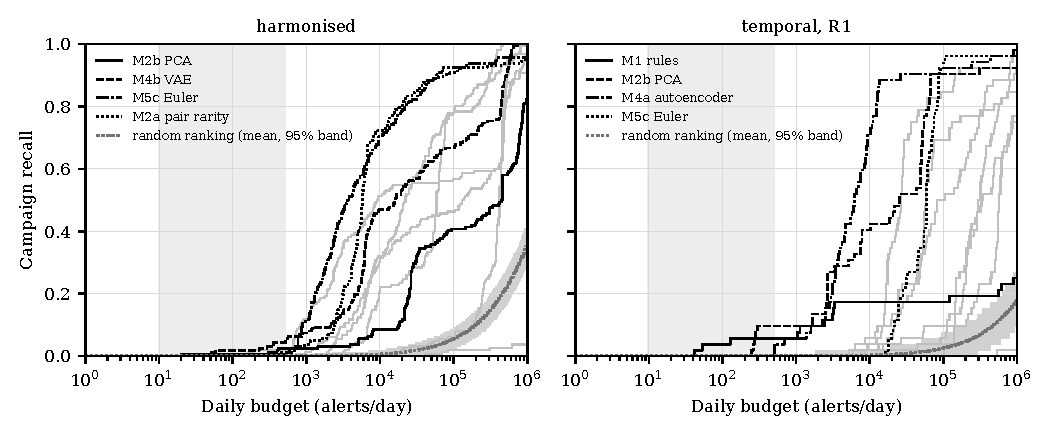
\includegraphics[width=\textwidth]{generated/figure_campaign_recall.pdf}
\caption{Campaign recall as a function of the daily budget in events, from each campaign's detection budget $b(c)$; arrival tie order. Black: four detectors named in the text; grey: the other non-floor detectors; shaded: 10 to 500 alerts per day.}
\label{fig:recall}
\end{figure}

\subsection{Within 500 events per day}
\label{sec:within}
No detector detects a campaign at 10 alerts per day in either protocol. In the harmonised protocol, the best recall at 500 is \HarmVaeRecallFiveHundred{} (the VAE), and PCA, the VAE and the autoencoder are the only detectors to catch a campaign at 50 or 100. A random ranking detects a campaign within 500 alerts with probability \HarmNullWithinFiveHundred{} there and \TempNullWithinFiveHundred{} in the temporal test, whose days are larger. In the temporal protocol, PCA reaches \TempPcaRecallFiveHundred{} at 500 and M1 catches campaigns from 50 alerts per day (\TempRulesRecallFifty{}, \TempRulesRecallHundred{} and \TempRulesRecallFiveHundred{} at 50, 100 and 500).

\subsection{First detection against the random-ranking null}
In the harmonised protocol, PCA (\HarmPcaFirstDetection{} alerts per day), the VAE (\HarmVaeFirstDetection{}) and the autoencoder (\HarmAutoencoderFirstDetection{}) reach a first detection that a random ranking matches with probability \HarmPcaNullP{}, \HarmVaeNullP{} and \HarmAutoencoderNullP{}; Euler (\HarmEulerFirstDetection{}, \HarmEulerNullP{}) and pair rarity (\HarmPairRarityFirstDetection{}, \HarmPairRarityNullP{}) follow. HBOS, with the highest ROC-AUC of the protocol (\HarmHbosRocAuc{}), first detects at \HarmHbosFirstDetection{} (\HarmHbosNullP{}). In the temporal protocol, M1 first detects at \TempRulesFirstDetection{} (\TempRulesNullP{}), PCA at \TempPcaFirstDetection{} (\TempPcaNullP{}) and the autoencoder at \TempAutoencoderFirstDetection{} (\TempAutoencoderNullP{}); Euler, with ROC-AUC \TempEulerRocAuc{}, first detects at \TempEulerFirstDetection{}, which a random ranking matches with probability \TempEulerNullP{}. These probabilities are per detector and not adjusted for the comparison of thirteen; each $b^{*}$ is determined by one campaign of one operation, and its interval is one-sided (\cref{sec:uncertainty}).

\subsection{Orderings induced by threshold-free and low-false-positive-rate metrics}
\label{sec:orderings}
\Cref{tab:correlations} compares, over the non-trivial detectors (\HarmNonTrivial{} harmonised, M1 being identical to M1u, and \TempNonTrivial{} temporal), the ordering induced by each metric with the ordering by first-detection budget. ROC-AUC does not track it in either protocol ($\rho = \HarmSpearmanRocAuc$ and $\TempSpearmanRocAuc$). AUC-PR tracks it weakly in the temporal protocol and not in the harmonised one, and recall at a false-positive rate of $10^{-4}$ tracks it best ($\rho = \TempSpearmanRecallFpr$, $p = \TempSpearmanPRecallFpr$, in the temporal protocol). The agreement of AUC-PR and low-false-positive-rate recall with the first-detection budget is close to definitional, since all three are governed by the best-ranked positives, whereas ROC-AUC is a mean-rank statistic; that the agreement is weak in the harmonised protocol, where the test spans 57 days, shows that even those metrics pool days that a daily queue keeps apart.

\begin{table}[t]
\centering
\small
\begin{threeparttable}
\caption{Spearman correlation between each metric and the first-detection budget (lower is better, so a positive $\rho$ means agreement) over the non-trivial detectors, with two-sided Monte Carlo permutation $p$-values (\PermutationCount{} permutations).}
\label{tab:correlations}
\begin{tabular}{@{}lrrrr@{}}
\toprule
& \multicolumn{2}{c}{Harmonised} & \multicolumn{2}{c}{Temporal} \\
Metric & $\rho$ & $p$ & $\rho$ & $p$ \\
\midrule
\tablerows{generated/table_correlations.tex}
\bottomrule
\end{tabular}
\end{threeparttable}
\end{table}

\subsection{Alert units}
\label{sec:units}
\Cref{tab:units} ranks the harmonised test in edge-hours and user-days. The picture changes: at 500 user-days per day, Euler reaches \HarmEulerUserDayFiveHundred{} of the campaigns and source rarity \HarmSourceRarityUserDayFiveHundred{}, against \HarmRandomUserDayFiveHundred{} for the random floor, and Euler catches \HarmEulerUserDayFifty{} at 50. Euler and source rarity have little event-level signal at the top of the queue but rank the compromised users' days high; Euler scores edges, so a user-day collects its highest edge, and source rarity is the user-source relation itself. The reverse holds for the rules: M1u's single early edge-hour detection does not carry over to user-days. Two cautions apply. A user-day budget of 500 covers a larger share of a day than 500 events, which is why the random floor is no longer at zero; and units carry no tie bracket, which matters for coarse scores such as M2a and M2c, whose top tier is shared by many events (\cref{sec:ties-results}). In the temporal protocol (\cref{app:units}), the same shift is smaller: at 500 user-days PCA and Euler reach \TempPcaUserDayFiveHundred{} and \TempEulerUserDayFiveHundred{}, against \TempRandomUserDayFiveHundred{} for the floor.

\begin{table}[t]
\centering
\footnotesize
\begin{threeparttable}
\caption{Harmonised protocol in three alert units, and with a fixed threshold. Campaign recall at 500 events, 500 edge-hours, 50 and 500 user-days per day; $b^{*}$ in user-days; alerts raised per test day, mean and maximum, by the threshold calibrated on training for 10 alerts per day.}
\label{tab:units}
\setlength{\tabcolsep}{4pt}
\begin{tabular}{@{}lrrrrrrr@{}}
\toprule
& Events & Edge-hours & \multicolumn{3}{c}{User-days} & \multicolumn{2}{c}{Fixed threshold, 10/day} \\
Detector & @500 & @500 & @50 & @500 & $b^{*}$ & mean & max \\
\midrule
\tablerows{generated/table_units_harm.tex}
\bottomrule
\end{tabular}
\end{threeparttable}
\end{table}

\subsection{A threshold fixed in advance}
\label{sec:fixed-results}
Calibrated on the harmonised training hours for 10 alerts per day, the thresholds do not transfer (\cref{tab:units}): PCA raises \HarmPcaFixedTenMean{} alerts per test day on average and \HarmPcaFixedTenMax{} on its worst day, the VAE \HarmVaeFixedTenMean{} and \HarmVaeFixedTenMax{}, and pair rarity, whose threshold falls inside a tie, \HarmPairRarityFixedTenMean{}; HBOS raises fewer than asked (\HarmHbosFixedTenMean{}). Forty-one hours of training do not describe the following eight weeks. Calibrated on three validation days, the temporal thresholds overshoot less: PCA raises \TempPcaFixedTenMean{} alerts per day on average and M1 \TempRulesFixedTenMean{}, while pair rarity, source rarity and Isolation Forest raise almost none (\TempPairRarityFixedTenMean{}, \TempSourceRarityFixedTenMean{} and \TempIForestFixedTenMean{}; \cref{app:units}).

\subsection{Regimes}
\Cref{tab:regimes} lists the temporal detectors whose AUC-PR or first detection moves by more than 1\% when the \TempTrainPositives{} training red-team events are removed from the fitted rows (R2); the other \RegimeUnchanged{} do not. Removing them moves Euler's first detection from \TempEulerFirstDetection{} to \TempTwoEulerFirstDetection{}, Isolation Forest's from \TempIForestFirstDetection{} to \TempTwoIForestFirstDetection{}, and the autoencoder's from \TempAutoencoderFirstDetection{} to \TempTwoAutoencoderFirstDetection{} with its ROC-AUC from \TempAutoencoderRocAuc{} to \TempTwoAutoencoderRocAuc{}; no conclusion of \cref{sec:within} changes. The \TempTrainPositives{} red-team events among \TempTrainEvents{} training events are enough to move these detectors in either direction; we do not interpret the direction.

\begin{table}[t]
\centering
\small
\begin{threeparttable}
\caption{Temporal protocol: detectors whose AUC-PR or first-detection budget changes by more than 1\% between R1 (red-team events in the fitted rows) and R2 (removed).}
\label{tab:regimes}
\begin{tabular}{@{}lllrrrr@{}}
\toprule
& \multicolumn{2}{c}{AUC-PR} & \multicolumn{2}{c}{ROC-AUC} & \multicolumn{2}{c}{$b^{*}$} \\
Detector & R1 & R2 & R1 & R2 & R1 & R2 \\
\midrule
\tablerows{generated/table_regimes.tex}
\bottomrule
\end{tabular}
\end{threeparttable}
\end{table}

\subsection{What the test bootstrap does not see}
\label{sec:variance}
\Cref{tab:fit-variance} refits the seeded detectors with five seeds. In the harmonised protocol, PCA's first detection ranges from \HarmPcaFitFirstMin{} to \HarmPcaFitFirstMax{} alerts per day and its AUC-PR varies by a factor of almost four; Isolation Forest's from \HarmIForestFitFirstMin{} to \HarmIForestFitFirstMax{}. PCA's position as the earliest harmonised detector is therefore a property of one fit. In the temporal protocol, where PCA retains less variance after tuning, its first detection stays between \TempPcaFitFirstMin{} and \TempPcaFitFirstMax{}, while Isolation Forest's spans \TempIForestFitFirstMin{} to \TempIForestFitFirstMax{}. With source users as the resampling unit, \HarmUserClusterSignificant{} of the 78 pairwise AUC-PR differences remain significant in the harmonised protocol (against \HarmPairsSignificant{} with benign events as singletons) and \TempUserClusterSignificant{} in the temporal one (against \TempPairsSignificant{}): benign correlation widens the intervals enough to change verdicts.

\begin{table}[t]
\centering
\footnotesize
\begin{threeparttable}
\caption{Range over five fitting seeds of AUC-PR, first-detection budget and campaign recall at 500 alerts per day, tuned configuration fixed.}
\label{tab:fit-variance}
\begin{tabular}{@{}llllr@{}}
\toprule
Protocol & Detector & AUC-PR & $b^{*}$ & @500 \\
\midrule
\tablerows{generated/table_fit_variance.tex}
\bottomrule
\end{tabular}
\end{threeparttable}
\end{table}

\subsection{Ties and campaign definition}
\label{sec:ties-results}
Pair rarity anchors its denominator to the start of the day, so equally new pairs tie: in the harmonised protocol \HarmPairRarityContenders{} events compete for the last places of the 500-alert budget over the test days. Under arrival order its campaign recall is the one reported; the most favourable order would give \HarmPairRarityBracketTen{} at 10 alerts per day and \HarmPairRarityBracketFiveHundred{} at 500 (temporal: \TempPairRarityBracketTen{} and \TempPairRarityBracketFiveHundred{}). That end of the bracket needs an oracle among tens of thousands of tied events, so it bounds what the tie hides rather than measuring the detector. Regrouping the harmonised positives into campaigns at 1, 6, 24 and 72 hours gives \HarmGapCampaignsOne{}, \HarmGapCampaignsSix{}, \HarmGapCampaignsTwentyFour{} and \HarmGapCampaignsSeventyTwo{} campaigns (temporal: \TempGapCampaignsOne{}, \TempGapCampaignsSix{}, \TempGapCampaignsTwentyFour{}, \TempGapCampaignsSeventyTwo{}); campaign recall therefore depends on a threshold that the data do not fix. The regrouping sees only the partition's positives, which is why it gives \HarmGapCampaignsTwentyFour{} rather than \HarmTestCampaigns{} campaigns at 24 hours.

\section{Diagnostics}
\label{sec:diagnostics}

\paragraph{The rule engine, rule by rule.} With uniform weights, M1u ranks the red team below benign traffic (ROC-AUC \TempRulesUniformRocAuc{} in the temporal protocol and \HarmRulesUniformRocAuc{} in the harmonised one). \Cref{tab:rules-lanl} scores each rule on every malicious test event and a seeded one-in-25 hash sample of benign events (\TempRuleSampleBenign{} and \HarmRuleSampleBenign{} benign events), which leaves ROC-AUC unbiased. In the temporal protocol \TempRulesBelowChance{} rules, and in the harmonised one \HarmRulesBelowChance{}, give the red team a ROC-AUC below 0.5. The largest effect is R5, which scores the rarity of pairs only for machine accounts: \TempMachineBenignShare{} (temporal) and \HarmMachineBenignShare{} (harmonised) of benign events have a machine account as source user, and none of the red-team events do. R3 and R4 also point the wrong way: malicious events have fewer recent failures on their destination than benign ones, and occur at hours closer to their user's usual ones. Only R1 (a new user-destination pair) carries a clear signal. On the temporal protocol, tuning the weights on validation labels turns the same rules into the detector with the earliest first detection (\TempRulesFirstDetection{} alerts per day), with labels from the same operation (\cref{sec:threats}).

\begin{table}[t]
\centering
\small
\begin{threeparttable}
\caption{ROC-AUC of each rule of M1 on the test partitions: malicious events against a one-in-25 sample of benign events.}
\label{tab:rules-lanl}
\begin{tabular}{@{}lrr@{}}
\toprule
Rule & Temporal & Harmonised \\
\midrule
\tablerows{generated/table_rules_lanl.tex}
\bottomrule
\end{tabular}
\end{threeparttable}
\end{table}

\paragraph{The source side.} \TopHost{} is the source of \RedTeamTopHostShare{} of the red-team events. The catalogue now describes the source computer (M2c and rule R8, and the F3 relations), and source rarity ranks the compromised users' days among the highest (\cref{sec:units}), in line with the source-side rule of \textcite{garchery2020adsage}. At the event level it does not (first detection at \HarmSourceRarityFirstDetection{} alerts per day in the harmonised protocol).

\section{Euler: reproduction and reconciliation}
\label{sec:euler}

\paragraph{Fidelity check.} We ran our reimplementation under the paper's own protocol: training before the first red-team event, edges scored per 30-minute snapshot, and edge-level AUC and average precision (AP) compared with table VI of \textcite{king2022euler} (GCN with GRU, link prediction). \Cref{tab:euler} gives four configurations over five seeds each: all events; NTLM authentications only, as the authors' loader keeps; that subset with the authors' node vocabulary (every computer has its own identifier, including those first seen after training); and with their default learning rate and patience. None reaches the published values: the NTLM subset gives AUC \EulerFidNtlmAuc{} and AP \EulerFidNtlmAp{}.

\paragraph{The authors' code.} We then ran the authors' code (\texttt{iHeartGraph/Euler}, commit \texttt{b6ab8fd}), edited only where its instructions ask for paths, with its pinned dependencies, on the same machine and data, five repetitions. It reproduces the published AUC closely (\EulerAuthorsAuc{} $\pm$ \EulerAuthorsAucSd{}) but not the published AP: \EulerAuthorsAp{} $\pm$ \EulerAuthorsApSd{}, between \EulerAuthorsApMin{} and \EulerAuthorsApMax{} over the five runs, against \EulerPublishedAp{}. Our reimplementation remains below the authors' code by about three points of AUC and half the AP. Their code contains choices that the paper does not describe and that we do not reproduce: ten negative samples per edge in training, early stopping on the sum of validation AUC and AP, dropout 0.25 with edge dropout 0.8, and one optimiser step per epoch over the whole training sequence. Which of them closes the gap is not tested here.

\begin{table}[t]
\centering
\footnotesize
\begin{threeparttable}
\caption{Euler, edge-level link prediction under the authors' protocol: mean $\pm$ standard deviation over five seeds or repetitions.}
\label{tab:euler}
\setlength{\tabcolsep}{3pt}
\begin{tabular}{@{}L{4.1cm}rlll@{}}
\toprule
Configuration & Events & Test edges (anomalous) & AUC & AP \\
\midrule
\tablerows{generated/table_euler.tex}
\bottomrule
\end{tabular}
\end{threeparttable}
\end{table}

\paragraph{The test sets, edge by edge.} The comparison is between implementations on the same data, not between datasets. Recounted in our snapshot alignment (multiples of 30 minutes), the authors' prepared files give exactly our NTLM test set: \EulerTestEdges{} edges, of which \EulerOurAlignmentAnomalous{} anomalous plus the first red-team event, which their preprocessing skips as if it were a header line and labels benign. Their loader aligns snapshots on the start of the test instead, which gives \EulerTheirAlignmentEdges{} edges and \EulerTheirAnomalous{} anomalous ones, \EulerPublishedAnomalous{} with the skipped line, the count of the paper's table V; it drops the \EulerTheirLastSnapshot{} edges of the last, partial snapshot. Their predictor never scores the first test snapshot, which holds \EulerAuthorsFirstSnapshot{} anomalous edges, so \EulerAuthorsEvaluated{} anomalous edges are evaluated in every repetition. Every count in this paragraph was recomputed with the authors' own loader or from their files.

\section{Comparison with published budgeted results}
\label{sec:comparison}
\Cref{tab:comparison} places the case study next to published budgeted results on the same data. They differ from ours in event universe, alert unit and split, and none was produced under our protocol, so the table states what each number measures rather than ranking them. The user-day unit brings our numbers closest to those of \textcite{garchery2020adsage}, whose source-side rule we now include: like them, we find that a source-novelty score detects a substantial share of the campaigns at budgets of hundreds of user-days per day. At the event level, our zeros at 10 alerts per day remain.

\begin{table}[t]
\centering
\footnotesize
\begin{threeparttable}
\caption{Published budgeted results on LANL and the present case study. Units and universes differ; numbers are not comparable across rows.}
\label{tab:comparison}
\begin{tabular}{@{}L{3.1cm}L{4.1cm}L{2.2cm}L{4.5cm}@{}}
\toprule
Work & Universe and split & Alert unit & Reported result \\
\midrule
\textcite{larroche2021decades} & LogOn events with user destination; train 8 days, test next 5 & events per day & DR-1K = 0.081 (DECADES) \\
\textcite{garchery2020adsage} & authentications without system accounts; train days 1--8, test 9--13 & user-days & CR-1000 = 0.254 for the \enquote{known source pc} rule, 0.255 for ADSAGE \\
\textcite{larroche2025ultralmd} & remote authentications and network flows as host-host edges, hourly windows & edges per hour & Rec@10 = 0.1788 (UltraLMD++, after removing duplicate lateral-movement edges) \\
This case study, harmonised & remote LogOn; train hours 0--41, test 41--1392 & events, user-days per day & events: no campaign at 10, \HarmVaeRecallFiveHundred{} at 500 (M4b); user-days: \HarmEulerUserDayFiveHundred{} (M5c) and \HarmSourceRarityUserDayFiveHundred{} (M2c) at 500 \\
\bottomrule
\end{tabular}
\end{threeparttable}
\end{table}

\section{A control for circularity}
\label{sec:circularity}

Before the LANL runs, the protocol was exercised on a synthetic sample whose generator emits each campaign as a chain: a user authenticates from $A$ to $B$, then from $B$ to $C$. On that sample, the rule engine detects all four test campaigns at 10 alerts per day. A decomposition by rule (\cref{tab:rules}) explains why: rule R7, which tests whether a user's previous destination equals the current source within 30 minutes, is the generator's own predicate; it separates malicious from benign events by a factor of \DemoRSevenRatio{} and receives a calibrated weight of \DemoRSevenWeight{}. On LANL, the same rule ranks the red team at or below chance (\cref{tab:rules-lanl}). A synthetic sample written by the author of the rules cannot distinguish a good heuristic from one informed by the generator.

\begin{table}[t]
\centering
\small
\begin{threeparttable}
\caption{Rule-level discrimination on the synthetic sample: mean raw rule score on benign and malicious events, their ratio, and the weight calibrated on validation.}
\label{tab:rules}
\begin{tabular}{@{}lrrrr@{}}
\toprule
Rule & Benign & Malicious & Ratio & Weight \\
\midrule
\tablerows{generated/table_rules_demo.tex}
\bottomrule
\end{tabular}
\begin{tablenotes}\footnotesize
\item A ratio of 0.0 means the rule never fired on a malicious event.
\end{tablenotes}
\end{threeparttable}
\end{table}

\section{Threats to validity}
\label{sec:threats}

\paragraph{One operation.} The labelled activity is one intrusion, mostly from one host (\cref{sec:concentration}). The bootstrap resamples the accounts of that operation; generalisation to other intrusions is not established, and every $p$-value should be read as stability under resampling of those accounts.

\paragraph{Labels and tuning.} In the temporal protocol, M1's weights are tuned on validation labels of the same operation, which \textcite{larroche2026fair} advises against; M1u and the harmonised protocol, which read no label, bound what that tuning adds. The other tunable detectors receive equal budgets, but the autoencoders and Euler keep their defaults, and in the harmonised protocol nothing is tuned.

\paragraph{Fitting variance.} Five seeds change some first-detection budgets by an order of magnitude (\cref{sec:variance}); the autoencoders and Euler were fitted once, so their position may move as much.

\paragraph{Units, ties and budgets.} Unit rankings carry no tie bracket; event rankings carry one, and only M2a and M0b have brackets of non-zero width. The staffing model behind the budgets rests on weak inputs. The fixed-threshold variant shows that a top-$k$ budget is an idealisation.

\paragraph{Features.} For a user's first event, the deviation from the user's typical hour is set to zero, the most typical value. The temporal training partition begins at day 0 without history, while validation and test have a warm-up.

\paragraph{Campaign definition and rule mapping.} Campaign recall depends on the grouping threshold (\cref{sec:ties-results}) and counts each compromised account of the operation as a campaign. The ATT\&CK techniques attached to the rules (\cref{app:rules}) express design intent and are not validated against ground truth.

\paragraph{External validity.} One enterprise network observed in 2015, before widespread multi-factor authentication; labels are a partial ground truth; the red team did not attempt to evade these detectors; and the raw files come from a mirror whose content, not whose compressed bytes, was verified.

\section{Scope of the claims}
\label{sec:scope}
For these detectors, universes and protocols, on one network and one operation: no campaign is detected within 10 events per day, at most a tenth within 500; several detectors reach a first detection that a random ranking rarely matches, and their ROC-AUC did not indicate which; and in user-days a graph detector and a source-novelty score reach about half of the campaigns at 500 per day. The results do not show that ROC-AUC fails to predict budgeted detection in general, that any detector family is better than another beyond this operation, or that Euler's published average precision is wrong: they show that its authors' code, on this data, does not reach it.

\section{Reproducibility}
\label{sec:reproducibility}
The code, configuration and run outputs are public at \url{https://github.com/SaniAdamou14/AuthBench} \parencite{authbenchsoftware}; the first version of this report is archived \parencite{authbenchpreprint}. Continuous integration runs linting, strict type checking and the test suite on every change, regenerates the synthetic results byte for byte, and regenerates every number, table and figure of this report from the committed run outputs, failing if a number or table differs. The evaluated run was produced by the code at commit \texttt{bd833eb} on a rented machine with 16 virtual CPUs and 61\,GB of memory in \RunHours{} hours from start to the last evaluation; its outputs, logs, the authors' Euler results and every recount quoted in \cref{sec:euler} are committed under \texttt{reports/runs/20261022T102638Z}. Fitting and resampling are seeded.

\section{Conclusion}
\label{sec:conclusion}
Under a leak-free protocol and at the event level, none of thirteen detectors detects a campaign of the LANL red team within 10 alerts per day, and ROC-AUC did not indicate which of them detect one earliest. Three findings qualify that statement more than any choice of detector: the alert unit (in user-days, a graph detector and a source-novelty score reach half of the campaigns at 500 per day), the fit (another seed moves a first detection by an order of magnitude), and the threshold (calibrated on 41 hours, it does not hold for eight weeks). The reproduction of Euler adds a fourth: the authors' own code does not reach its published average precision on the published data. Because the labelled activity is one operation, these findings describe one case; the harness is meant to make the next case cheap to evaluate.

\section*{Ethics and data statement}
\addcontentsline{toc}{section}{Ethics and data statement}
The LANL data are public and de-identified, and their use requires citation of the provider; the benchmark manipulates no personal data. It is defensive in purpose and contains no offensive technique. The authors' Euler code carries no licence; it was run unmodified apart from paths, and only those path edits are published with the run outputs.

% References and appendices each start on a page of their own.
\clearpage
\printbibliography[heading=bibintoc]

\clearpage
\appendix

\section{Features}
\label{app:features}
\begin{table}[h]
\centering
\footnotesize
\begin{tabular}{@{}llp{6.4cm}@{}}
\toprule
Family & Feature & Definition \\
\midrule
F1 & \texttt{is\_success} & Outcome of the authentication \\
F1 & \texttt{auth\_type\_is\_null}, \texttt{logon\_type\_is\_null} & Missingness indicators \\
F1 & \texttt{src\_user\_is\_machine} & Source user is a machine account \\
F1 & \texttt{src\_dst\_user\_same}, \texttt{src\_dst\_computer\_same} & Source and destination coincide \\
F1 & \texttt{domain\_crossing} & Source and destination domains differ \\
F1 & \texttt{*\_freq} (3) & Training-fitted relative frequency of the authentication type, logon type and orientation \\
F2 & \texttt{src\_user\_\{1h,1d\}\_n\_events} & Earlier events of the source user in the window $[t-w, t)$ \\
F2 & \texttt{src\_user\_\{1h,1d\}\_failure\_ratio} & Share of those events that failed \\
F3 & \texttt{pair\_is\_new}, \texttt{pair\_global\_rarity} & First occurrence and rarity of the (user, destination) pair \\
F3 & \texttt{user\_src\_is\_new}, \texttt{user\_src\_rarity} & The same for the (user, source) pair \\
F3 & \texttt{src\_dst\_is\_new}, \texttt{src\_dst\_rarity} & The same for the (source, destination) edge \\
F3 & \texttt{user\_new\_host\_count\_24h} & New pairs of the user over the preceding 24 hours \\
F3 & \texttt{host\_new\_user\_count\_24h} & New pairs of the destination over the preceding 24 hours \\
F4 & \texttt{hour\_sin}, \texttt{hour\_cos} & Time of day on the unit circle \\
F4 & \texttt{hour\_deviation\_from\_profile} & Angular distance to the circular mean of the user's earlier events (0 for a first event) \\
\bottomrule
\end{tabular}
\end{table}
M1 additionally reads columns outside the design matrix: the number of distinct destinations of the user in the past hour (R2), the number of failures on the destination in the past hour (R3), whether the user's authentication type is new (R6) and whether the user's previous event ended on the current source (R7).

\section{Rules of M1}
\label{app:rules}
\begin{table}[h]
\centering
\footnotesize
\begin{tabular}{@{}lp{9.0cm}l@{}}
\toprule
Rule & Raw signal & ATT\&CK \\
\midrule
R1 & The (user, destination) pair is new & T1078 \\
R2 & Distinct destinations of the user in the past hour above the user's training 99.9th percentile & T1078 \\
R3 & Failures on the destination in the past hour, counted when the current authentication succeeds & T1110 \\
R4 & Deviation from the user's typical hour & T1078 \\
R5 & Pair rarity, counted only for machine accounts & T1550 \\
R6 & First use of an authentication type by the user & T1550 \\
R7 & The user's previous event ended on the current source computer, within 30 minutes & T1021 \\
R8 & First use of a source computer by the user & T1021 \\
\bottomrule
\end{tabular}
\end{table}
Each rule's raw signal is mapped to $[0, 1]$ by its empirical CDF on a seeded sample of at most two million events of the last training day, so that an event's score does not depend on the other events scored. Technique identifiers follow \textcite{strom2018attack} and record design intent. Some mappings are loose: R2 is closer to discovery or fan-out than to T1078, R5 carries no evidence of alternate authentication material, and R6 matches T1550 only in the pass-the-hash case. R7 requires the same account on consecutive events and misses chains in which credentials change between hops.

\section{Alert units and fixed thresholds, temporal protocol}
\label{app:units}
\begin{table}[h]
\centering
\footnotesize
\setlength{\tabcolsep}{4pt}
\begin{tabular}{@{}lrrrrrrr@{}}
\toprule
& Events & Edge-hours & \multicolumn{3}{c}{User-days} & \multicolumn{2}{c}{Fixed threshold, 10/day} \\
Detector & @500 & @500 & @50 & @500 & $b^{*}$ & mean & max \\
\midrule
\tablerows{generated/table_units_temp.tex}
\bottomrule
\end{tabular}
\end{table}
Thresholds are calibrated on validation. A test day has between \TempUserDaysMin{} and \TempUserDaysMax{} user-days, and the random floor reaches a user-day first detection of \TempRandomUserDayFirst{}, so first detections in user-days separate the detectors less than in events.

\section{Earlier code on the same temporal partitions}
\label{app:earlier}
The previous version of this report evaluated \WideModels{} detectors on the same temporal partitions with the code of September 2026: only M1's rule weights tuned, on labels; M1 normalised by rank over the scored partition; PCA, Isolation Forest and HBOS at their defaults; rarity denominators growing within the day; and a campaign-level bootstrap with 2{,}000 resamples. The training and test partitions hold the same events and positives in both runs. PCA changes most: tuning on validation retained less variance than the default, and its first detection fell from \WidePcaFirstDetection{} to \TempPcaFirstDetection{} alerts per day. The run does not separate the effect of each code change.
\begin{table}[h]
\centering
\footnotesize
\setlength{\tabcolsep}{4pt}
\begin{tabular}{@{}lllrrrr@{}}
\toprule
& \multicolumn{2}{c}{AUC-PR} & \multicolumn{2}{c}{ROC-AUC} & \multicolumn{2}{c}{$b^{*}$} \\
Detector & September & October & September & October & September & October \\
\midrule
\tablerows{generated/table_earlier.tex}
\bottomrule
\end{tabular}
\end{table}

\end{document}
